% ==============================================================================
%
%                                    DVG303
%                  Objektorienterad design och programmering
%                                Laboration #1
%
% Author:   Jonas Sjöberg
%           Högskolan i Gävle
%           tel12jsg@student.hig.se
%           https://github.com/jonasjberg
%
% License:  Creative Commons Attribution-NonCommercial-ShareAlike 4.0
%           International.  See LICENSE.md for full licensing information.
% ==============================================================================

\section{Uppgift 3}\label{sec:uppg3}

\subsection{}\label{sec:uppg3a}
\subsubsection*{Frågeställning}
Betrakta nu modellen en gång till: Ser ni likheter när det gäller objektens
beteenden? Vilka är dessa? Ge en Beskrivning!

\subsubsection*{Lösning}



\subsection{}\label{sec:uppg3b}
\subsubsection*{Frågeställning}
Utöka nu klassdiagrammet en gång till: Lägg till minst ett interface som
deklarerar någon metod som passar till det som ni beskrev ovan. Låt klasserna
implementera interfacet ifall det passar!

\subsubsection*{Lösning}

%\begin{figure}[htbp]
\begin{sidewaysfigure}[ht]
\centering
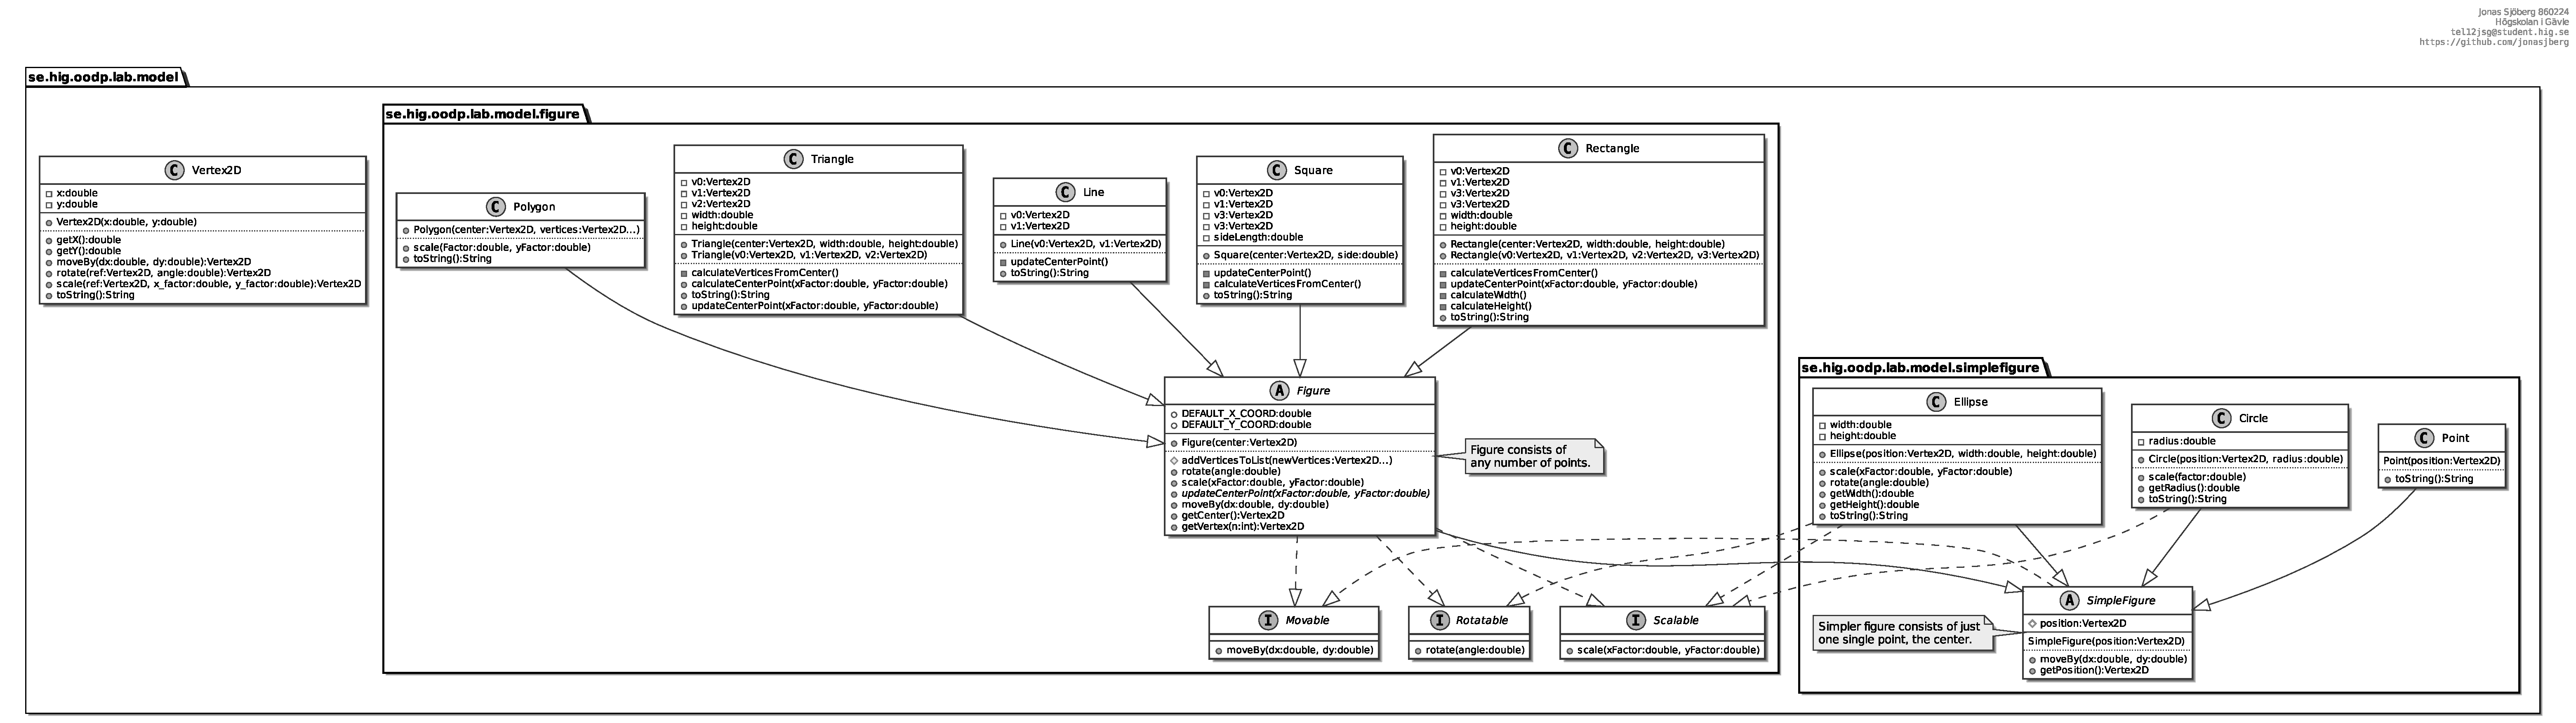
\includegraphics[width=\linewidth]{diagram/uppgift3.eps}
\caption{Uppgift~3\ref{sec:uppg2c}: UML-diagram för geometriska figurer
(\texttt{diagram/uppgift3.eps})}
\label{fig:uppg3a}
\end{sidewaysfigure}



\subsection{}\label{sec:uppg3c}
\subsubsection*{Frågeställning}
Uppdatera koden från uppgift 2 så att det motsvarar den utökade modellen från
(b)!

\subsubsection*{Lösning}


